\documentclass[]{article}

\usepackage{amsmath}
\usepackage{graphicx}
\usepackage{multicol}
\graphicspath{ {./results/} }

\title{Model CW}
\author{James Elgar}

\begin{document}

\maketitle

\section{Introduction}

In this report I will cover the use of least squares regression to estimate a
generalised model for a given set of data. I will first explain the process 
used to obtain the least squares for a given model and then explain how a
generalised model was selected and how cross validation was used to avoid overfitting. I will then show some results
from my code, displaying the 3 types of models used, polynomial (including
linear) up to order 5, exponential and sinusoidal.

\section{Regression}

The role of regression is to generate a model which represents the relationship
between the given data's independant variable and depent variable. Throughout
the code we used matrix form to calculate the model. This works by reducing the
error (residual) between the given values of $\boldsymbol{y}$ and the values of \boldsymbol{y} predicted by the model,
$\hat{\boldsymbol{y}}$. The predicted values of \boldsymbol{y} are caluated by mutiplying \boldsymbol{X} with the
caluated least squares, $\boldsymbol{a}$. $\boldsymbol{X}$ is formed by representing the terms from the
model, which for polynomial models is the Vandermonde matrix (shown below for
size n). 

\begin{equation}
  \boldsymbol{X} = 
  \begin{bmatrix}
    1   & x_1   & ... & {x_1}^n     \\
    1   & {x_2} & ... & {x_2}^n  \\
    ... & ...   & ... & ...     \\
    1   & {x_n} & ... & {x_n}^n  
  \end{bmatrix}
\end{equation}

For sin and exponential $\boldsymbol{X}$ would be:
\begin{multicols}{2}
  \begin{equation}
    \boldsymbol{X} = 
    \begin{bmatrix}
      1   & sin(x_1)        \\
      1   & sin(x_2)   \\
      ... & ...    \\
      1   & sin(x_n)   
    \end{bmatrix}
  \end{equation}\break
  \begin{equation}
    \boldsymbol{X} = 
    \begin{bmatrix}
      1     & e^{x_1}     \\
      1     & e^{x_2}  \\
      ...   & ...     \\
      1     & e^{x_n}  
    \end{bmatrix}
  \end{equation}
\end{multicols}

For a perfect model, $\boldsymbol{y} = \boldsymbol{\hat{y}} = \boldsymbol{Xa}$. However in most cases the given data
will not match perfectly to a model and therefore the aim is to reduce
the square error between the given $\boldsymbol{y}$ values and those predicted by our model.
The value for this error (residual) can be represetned by

\begin{equation}
  r = {\mid \mid \boldsymbol{y} - \boldsymbol{Xa} \mid \mid}^2
\end{equation}

Minimising this vector, gives the least squares for the model and can be
represetned by this foruma.

\begin{equation}
  \boldsymbol{a} = (\boldsymbol{X}^T \boldsymbol{X})^{-1}\boldsymbol{X}^T\boldsymbol{y}
\end{equation}

\section{Finding the best model}

When searching for the best model, we are looking for a model which is
generalised to the trend of the given data rather than the model with the lowest error. For a model to be
generalised it must represnt the trend of the data meaning adding more data
points from the same source would fit into the model. When a model is not
general but has a low error it is known as over-fitting. To avoid overfitting, the given data was seperated
into two groups, the training data and the testing data. The training data was
used to generate the least squares for each type of model (including different
numbers of features). The least squares
generated by the training data were then used to calculate the y values for the
testing set and the square error calculate by the following equation

\begin{equation}
  \sum\limits_{i=1} ({y_{i}} - \hat{y_{i}})^2
\end {equation}

where $y$ is the actual y values from the testing set and the $\hat{y}$ are
those calulated from the least squares generated by the training set. This
process of calulcating the error was repeated 50 times changing which points were
used for the training data and which were used for the testing data each time,
storing the total error for each type of model.
The model with the lowest total error would then give the most
generalised model for the given data as the error between
the newly added data from the same source (the testing data) was low.

\section{Results}

  \begin{figure}[!hbt]
    \centering
    \begin{minipage}[b]{0.45\textwidth}
      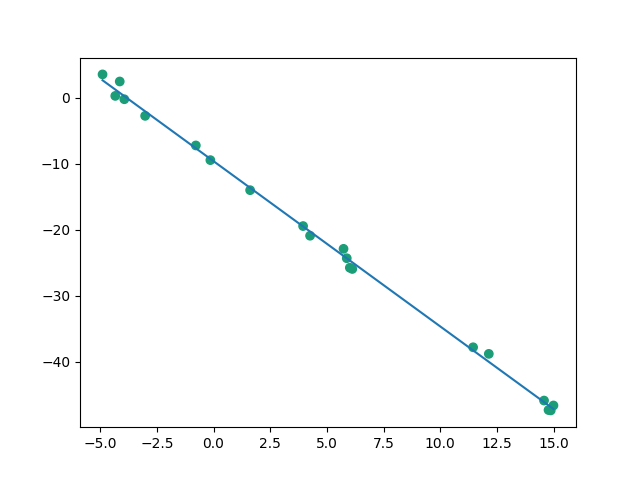
\includegraphics[width=\textwidth]{noise.png}
      \centering
      \caption {Results from data set noise1}
      \label{fig:noise1}
    \end{minipage}
    \hfill
    \begin{minipage}[b]{0.45\textwidth}
      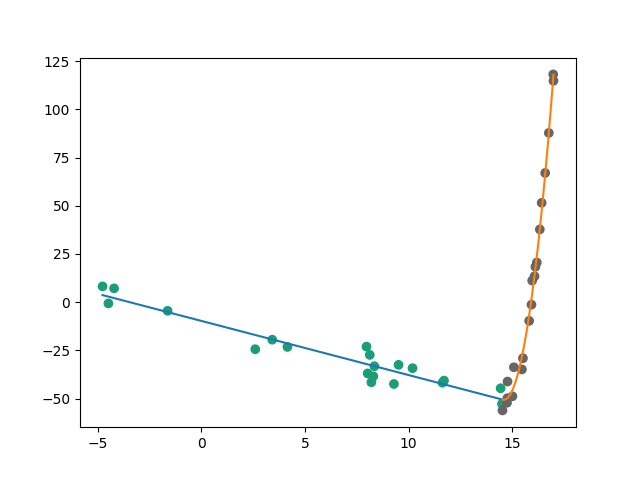
\includegraphics[width=\textwidth]{noise2.png}
      \caption {Results from data set adv1}
      \label{fig:noise2}
    \end{minipage}

  \end{figure}

  The results from \ref{fig:noise1} and \ref{fig:noise2}, demonstate the avoidance of overfitting. If
  the model with the lowest error was selected instead, we would expect a polynomial model with
  a higher number of features as this would more precisely map to the given points. Instead we get a higher error but a model which
  more generaly represents the trend of the given data.

\begin{figure}[!htb]
  \centering
  \begin{minipage}[b]{0.45\textwidth}
    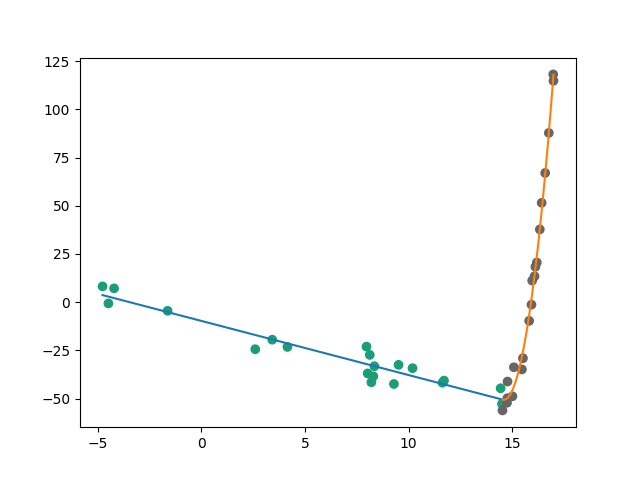
\includegraphics[width=\textwidth]{noise2.png}
    \caption {Results from data set noise2}
    \label{fig:noise2}
  \end{minipage}
  \hfill
  \begin{minipage}[b]{0.45\textwidth}
    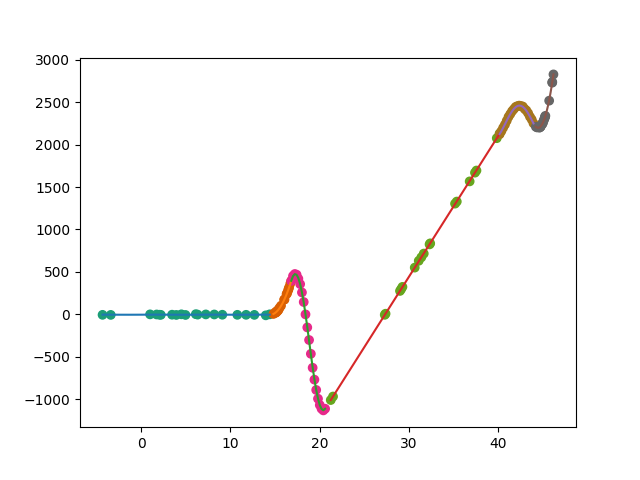
\includegraphics[width=\textwidth]{adv3.png}
    \caption {Results from data set adv3}
    \label{fig:adv3}
  \end{minipage}

\end{figure}


The results from \ref{fig:adv3}  and \ref{fig:noise2} show the use of different
types of models, other than the polynomial functions. In \ref{fig:adv3} the
third set of points is modeled by a sin function, which yields a slighly lower
error than using an order 3 polynomial in this case. It also allows for an
accurate model for a longer sinusoidal function, which would not be possible
with only polynomials up to order 5. Simialrly in
\ref{fig:noise2}, we see the use of an exponential model, in the second set of
points. \ref{fig:adv3} also demonstrates that getting a high error on a model
without noise is still possible. This is a result of the magnitude of the given
data, meaning even small deviations from the given dataset yields a large error.

\section{Conclusion}
The results from this report demonstrate the use of least squares to select
between 3 different types of model and then (in the case of polynomial) select
the model with the correct number of features for the best general fit for the data.
Using the process described in Section 1 and 2 the program could be extended to
select between additional models whilst ensuring overfitting is avoided.

\end{document}
